% --
% conclusion

\section{Conclusion}
\sectionheader{Conclusion}
\begin{frame}
  \frametitle{Signal Processing and Features}
  \begin{itemize}
    \item Conclusion based on the experiments of MFCC with CNNs:
    \begin{itemize}
      \item 32 MFCC coeff. were often worse than 12 MFCC coeff.
      \item frame-based normalization decreases the classification, but improves noise invariance as for selected conv-jim models:
      \vspace{-0.5cm}
      \begin{figure}[!ht]
        \centering
        \subfloat[\#MFCC: 12, Norm.: 0]{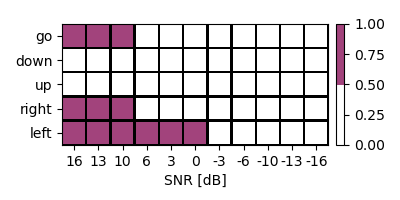
\includegraphics[width=0.3\textwidth]{../5_exp/figs/exp_fs_cepstral_tb_noise_conv-jim_mfcc12_norm0.png}}
        \qquad
        \subfloat[\#MFCC: 12, Norm.: 1]{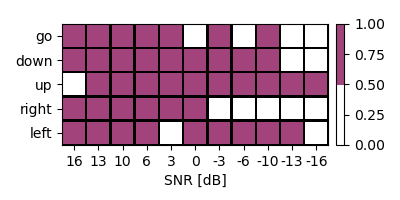
\includegraphics[width=0.3\textwidth]{../5_exp/figs/exp_fs_cepstral_tb_noise_conv-jim_mfcc12_norm1.png}}
      \end{figure}
      \item feature enhancements can improve the classification results, but double delta features are not really necessary.
    \end{itemize}
  \end{itemize}
\end{frame}


\begin{frame}
  \frametitle{Neural Network Models}
  Based on the Experiments one can conclude:
\end{frame}

\begin{frame}
  \Large
  \centering
  \vfill
  Thank you for your Attention
  \begin{quote}
    \scriptsize
    \vspace{1cm}
    \enquote{It is trivial to design a machine that learns very quickly, does not generalize, and requires an enormous amount of hardware.\\
    In fact this learning machine has already been built and is called a Random Access Memory.}\\
    \vspace{0.25cm}
    Y. LeCun
  \end{quote}
\end{frame}